\chapter{Popis navržených řešení}

V předešlé kapitole byla vysvětlena základní problematika, která souvisí s virtualizací síťových funkcí, cloud computingem a softwarově definovanými sítěmi. Zároveň byla popsána referenční architektura frameworku pro virtualizaci síťových funkcí. Tato kapitola bude již věnována konkrétnímu příkladu využití virtuálních síťových funkcí v cloudovém prostředí. Nejprve zde popsána navržená architektura pro privátní cloudovou platformu využívající virtualizaci síťových funkcí, kterou mohou využívat všichni její uživatelé. Pro tuto cloudovou platformu a pro její uživatele byli navrženy dva příklady virtuálních síťových funkcí. U obou příkladů jsou uvedeny scénáře a způsob jakým jsou navrženy.

\section{Architektura navrženého řešení}

Architektura navrženého řešení byla implementována pomocí cloudové platformy OpenStack a SDN řešení OpenContrail. Obrázku č. \ref{fig:VNF_overview} znázorňuje tyto technologie v souvislosti s referenční architekturou popsanou v kapitole \ref{sub:architektura}. Je nutné říci, že obě technologie nezapadají přímo do jedné z částí referenční architektury. Naopak v některých případech se překrývají či některou část neimplementují vůbec.

\begin{figure}[h]
\begin{centering}
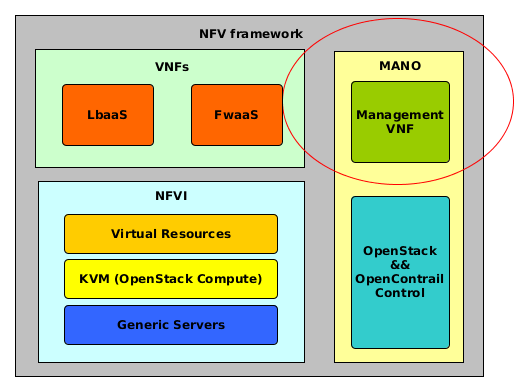
\includegraphics[scale=0.51]{images/VNF_overview}
\par\end{centering}
\caption{Architektura NFV řešení\label{fig:VNF_overview}}
\end{figure}

OpenStack byl zvolen, protože se jedná o největší open-source cloudovou platformu. OpenStack tvoří část správy infrastuktury. Hardwarová vrstva insfrastruktury se může skládat z libovolných serverů, na kterých KVM hypervizor. Tento hypervizor tvoří virtuální vrsvu a byl vybrán, protože je nejčastěji používán společně s OpenStackem. Avšak v případě potřeby by zde mohl být použit i jiný, pokud bude zachována kompatibilita vůči OpenStacku.

Speciálně pro vyřešení síťování v této infrastruktuře je součástí řešení OpenContrail. Díky tomu je možné vytvářet overlay sítě pomocí VXLAN či MPLSoverGRE, kterémi mohou být jednotlivé VM a VNF dynamicky spojovány.

Jednou z částí OpenStacku je i Heat engine. Ten bude v tomto návrhu zastávat roli VFN manager, pomocí kterého budou jednotlivé VNF spravováný.

Z toho návrhu je patrné, že zde není implementovaný NFV orchestrator. Je to zdůvodu toho, že pro účely řešení virtuálních síťových funkcí na cloudové platformě OpenStack s OpenContrailem, která je navržena v této práci, není tato čast potřeba. 


\section{Load balancer as a Service}

První VNF, která byla pro uživatele navržena, je Load balancing. 

Součástí OpenStacku je Neutron HAproxy. Ta může sloužit 

Obrázek + scénář
První síťovou funkcí, která může být  

\section{Firewall as a Service}

\subsection{Scénář NAT}

\subsection{Scénář Service Chaining}

\subsection{Scénář HA firewall}

\section{Heat Templates}

\begin{figure}[h]
\begin{centering}
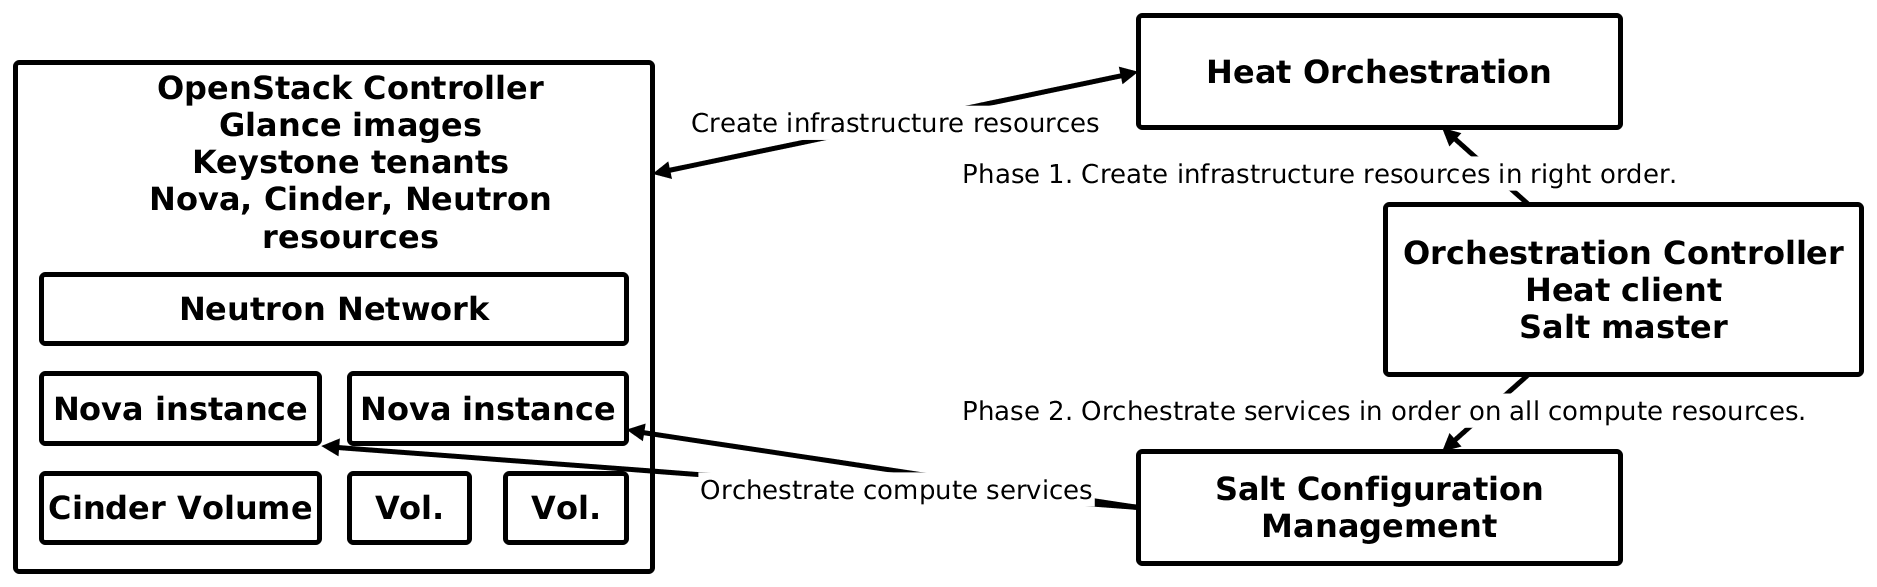
\includegraphics[scale=0.21]{images/heat}
\par\end{centering}
\caption{Popis heat orchestrace\label{fig:heat}}
\end{figure}

Popis co jsou to heat templates.

Heat is the main project of the OpenStack orchestration program. It allows users to describe deployments of complex cloud applications in text files called templates. These templates are then parsed and executed by the Heat engine.

\subsection{FwaaS template}

Pro FwaaS je narhnut heat template, který obsahuje:

\begin{itemize}
\item 1 firewall instanci
\item 1 testovaci instanci
\item 1 management instanci
\item management síť
\item privátní síť
\item contrail policy
\end{itemize}

\subsection{LbaaS template}

Navržený heat template pro LbaaS v sobě obsahuje následující prostředky, které se po spuštění pokusí vytvořit.

\begin{itemize}
\item pool
\item members
\item health monitoring
\item 2 web instance
\item privatni síť
\item public síť
\end{itemize}
